\documentclass[border = 1cm, preview, varwidth=\maxdimen]{standalone}

\usepackage{xeCJK}

% mathematics
\usepackage{amsmath}

% tikz
\usepackage{tikz}
\usepackage{ifthen}
\usetikzlibrary{arrows}
\usetikzlibrary{automata}
\usetikzlibrary{positioning}
\tikzset{->, > = stealth', node distance = 1in}

\begin{document}
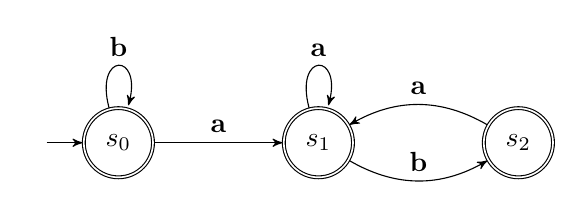
\begin{tikzpicture}
  % nodes
  \node [state, initial, accepting, initial text = ] (s0) {$s_0$};
  \node [state, accepting, right of = s0] (s1) {$s_1$};
  \node [state, accepting, right of = s1] (s2) {$s_2$};
  % paths
  \draw (s0) edge [loop above] node {\bf b} (s0);
  \draw (s0) edge [above] node {\bf a} (s1);
  \draw (s1) edge [loop above] node {\bf a} (s1);
  \draw (s1) edge [bend right, above] node {\bf b} (s2);
  \draw (s2) edge [bend right, above] node {\bf a} (s1);
\end{tikzpicture}
\end{document}
